\documentclass[tikz,border=5mm]{standalone}
\begin{document}
	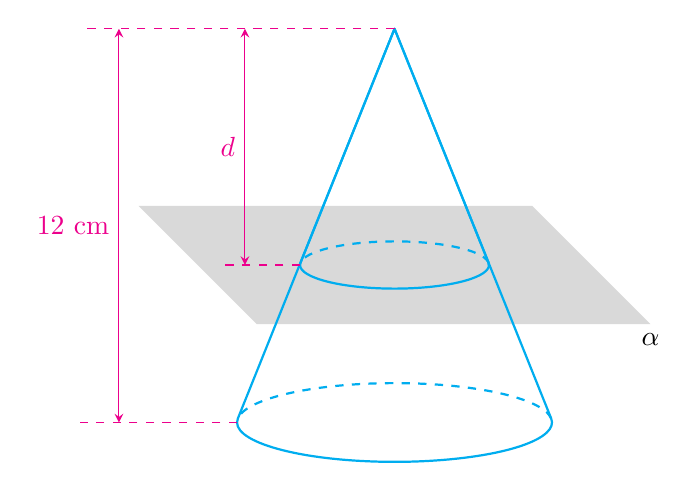
\begin{tikzpicture}[>=stealth,join=round]
		\def\a{2} % major
		\def\b{.5} % minor
		\def\h{5} % height of the cone
		\def\d{3} % height of the section
		\pgfmathsetmacro{\t}{asin(\b/\h)}
		\fill[gray!30,shift={(90:\h-\d)},scale=2.5,xslant=-1,yscale=.3] (-1,1) rectangle (1,-1) node[below,black]{$\alpha$};
		\begin{scope}[cyan,thick]
			\draw[dashed]
			(\t:{\a} and {\b}) arc(\t:180-\t:{\a} and {\b});
			\draw
			(\t:{\a} and {\b})--(0,\h)--(180-\t:{\a} and {\b})
			arc(180-\t:360+\t:{\a} and {\b});
			\begin{scope}[shift={(90:\h-\d)},scale={\d/\h}]
				\draw[dashed]
				(\t:{\a} and {\b}) arc(\t:180-\t:{\a} and {\b});
				\draw
				(\t:{\a} and {\b})--(0,\h)--(180-\t:{\a} and {\b})
				arc(180-\t:360+\t:{\a} and {\b})
				(-\a,0) coordinate (L);
			\end{scope}
		\end{scope}
		\begin{scope}[magenta]
			\draw[dashed] (-\a,0)--(-2*\a,0) (0,\h)--(-2*\a,\h)
			(L)--+(180:1) coordinate (Ld);
			\draw[<->] (-2*\a+.5,0)--+(90:\h) node[midway,left]{$12$ cm};
			\draw[<->] (Ld)++(0:.3)--+(90:\d) node[midway,left]{$d$};
		\end{scope}
	\end{tikzpicture}
\end{document}